%!TEX root = scivis_lbaakman_bvanloon.tex

\hypersetup{pageanchor=false}
\begin{titlepage}
    \centering
    \par\vspace{9cm}
    %{\scshape\LARGE University of Groningen \par}
          
            %\includegraphics[width=6cm]{img/logo.png} % also works with logo.pdf
    \par\vspace{3cm}
    {\huge\bfseries  Scientific Visualization \par}
    {\large\bfseries  An Interactive Application for Real-Time Simulation of Fluid Flow.\par}

    \vspace{2cm}\par
        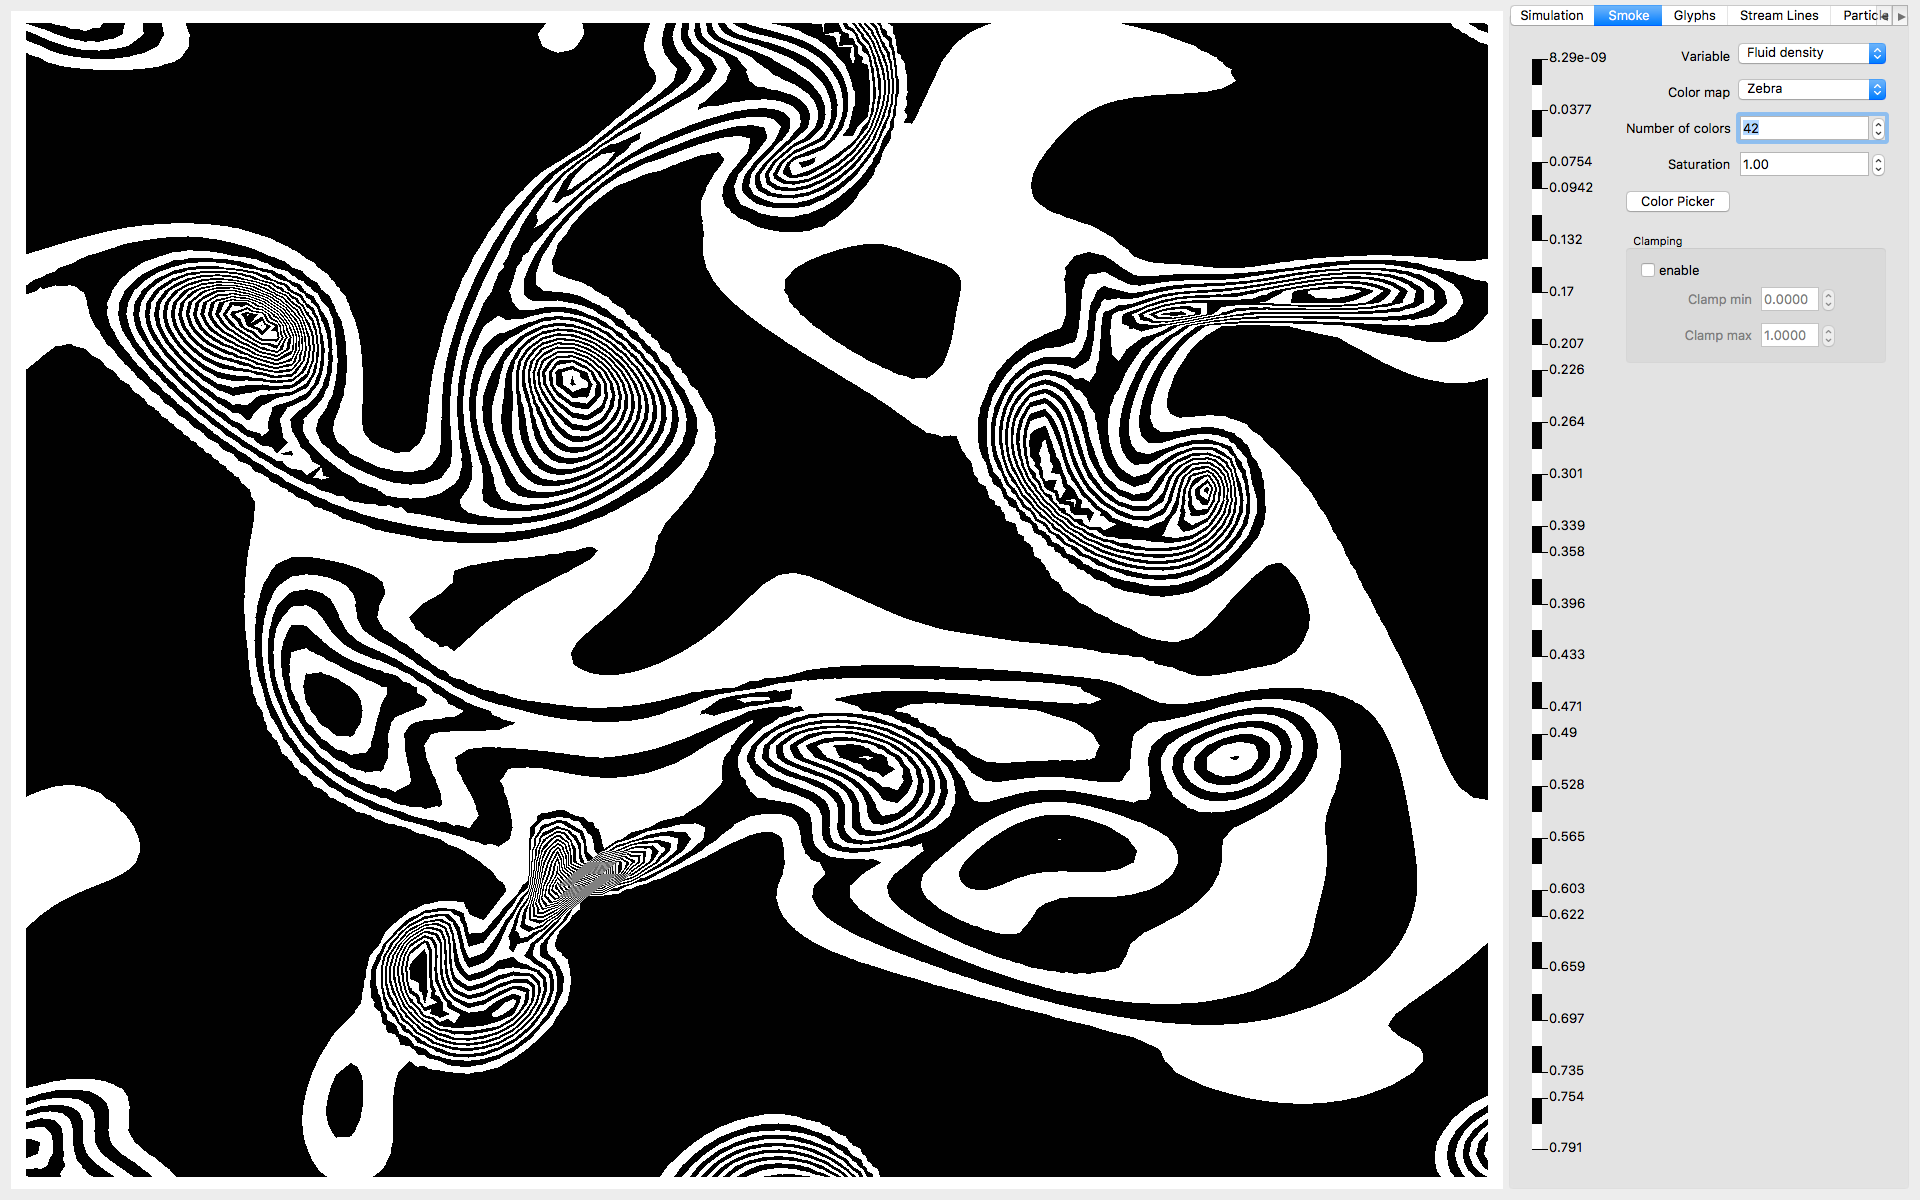
\includegraphics[width=0.42\textwidth, height=0.5\textheight, keepaspectratio=true]{img/titlepage/smoke.png} \hspace{10px}
        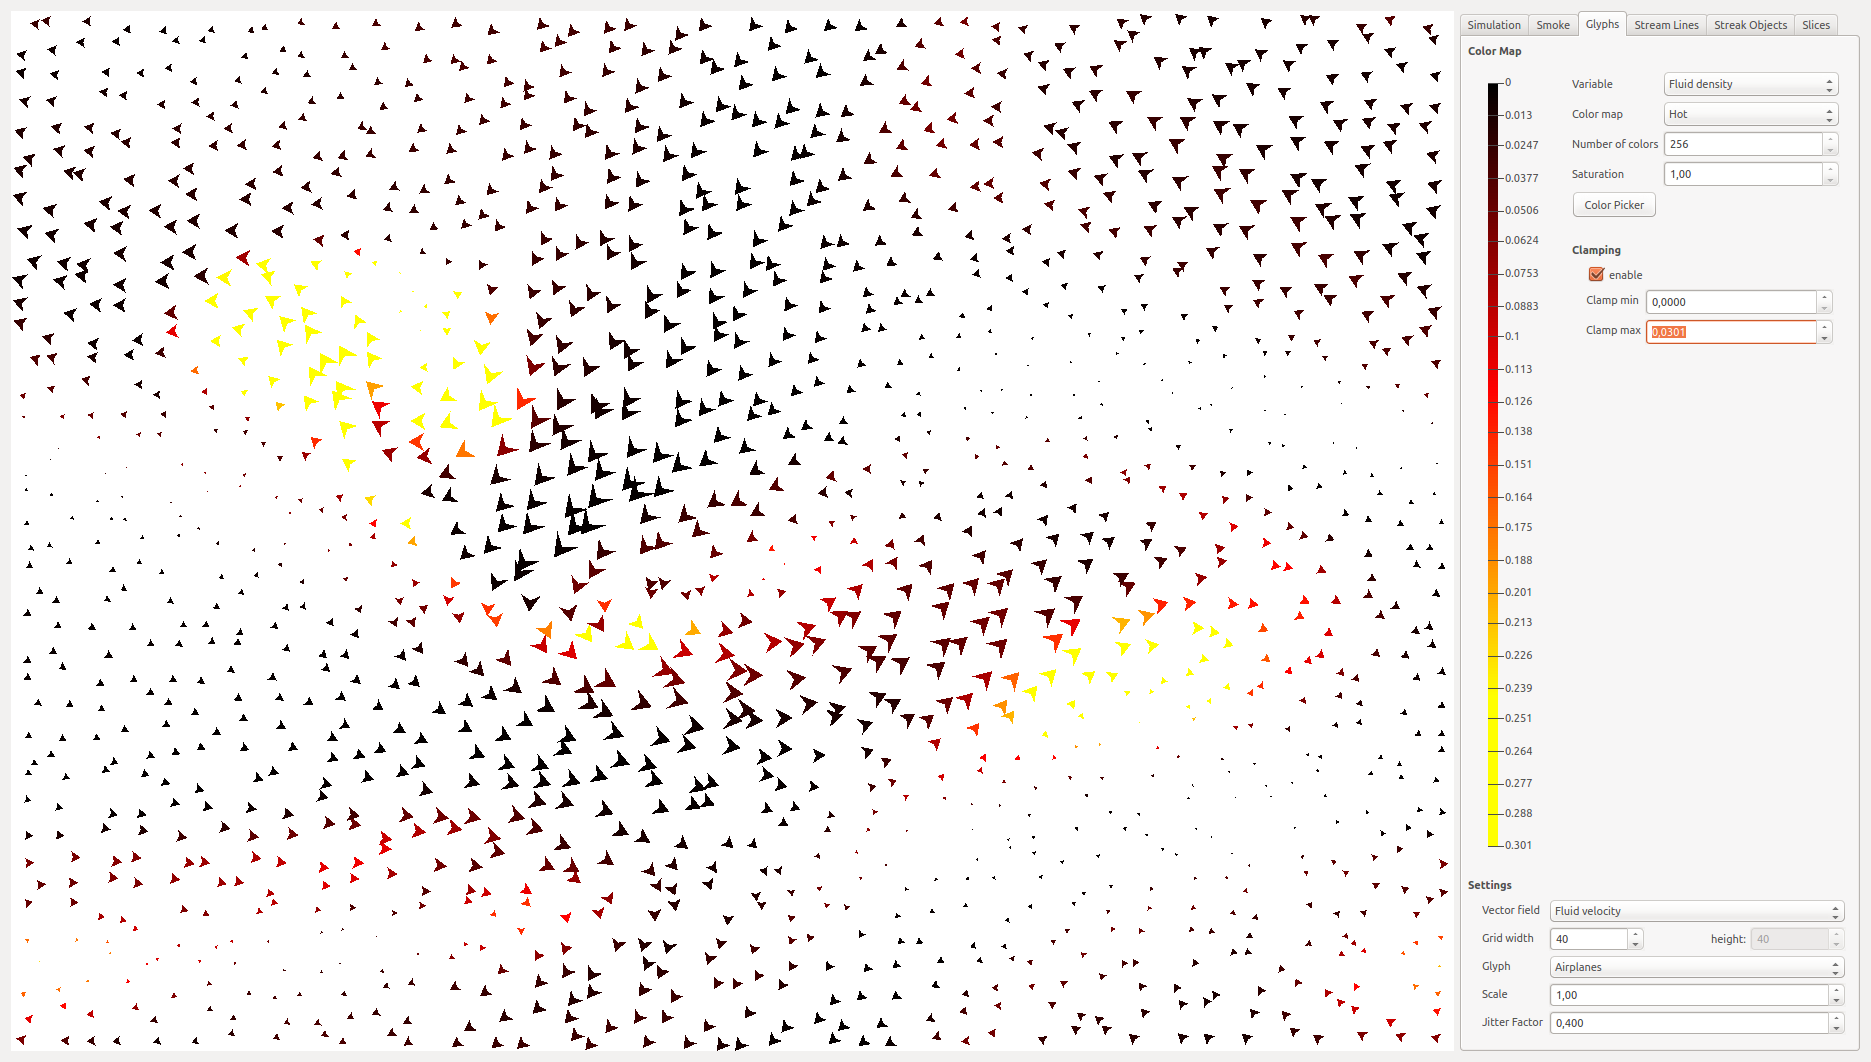
\includegraphics[width=0.42\textwidth, height=0.5\textheight, keepaspectratio=true]{img/titlepage/glyphs.png}

        \vspace{10px}
        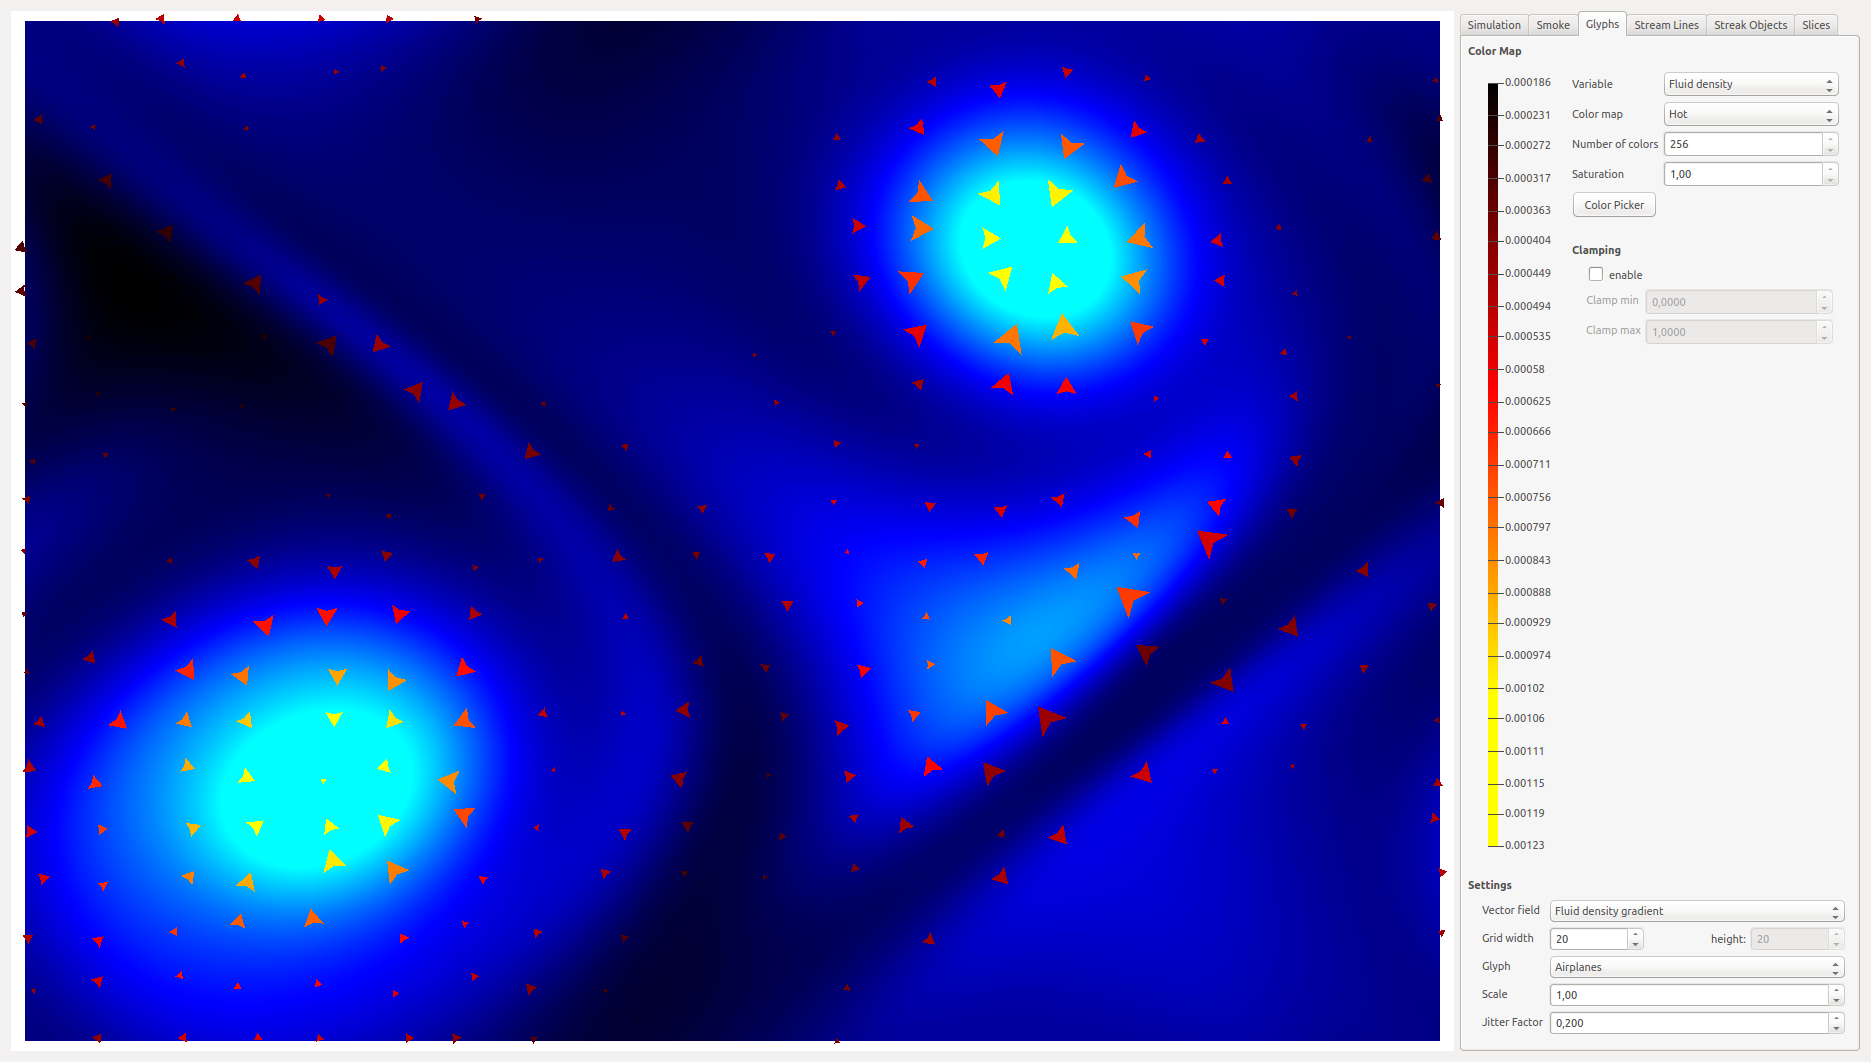
\includegraphics[width=0.42\textwidth, height=0.5\textheight, keepaspectratio=true]{img/titlepage/gradient.png} \hspace{10px}
        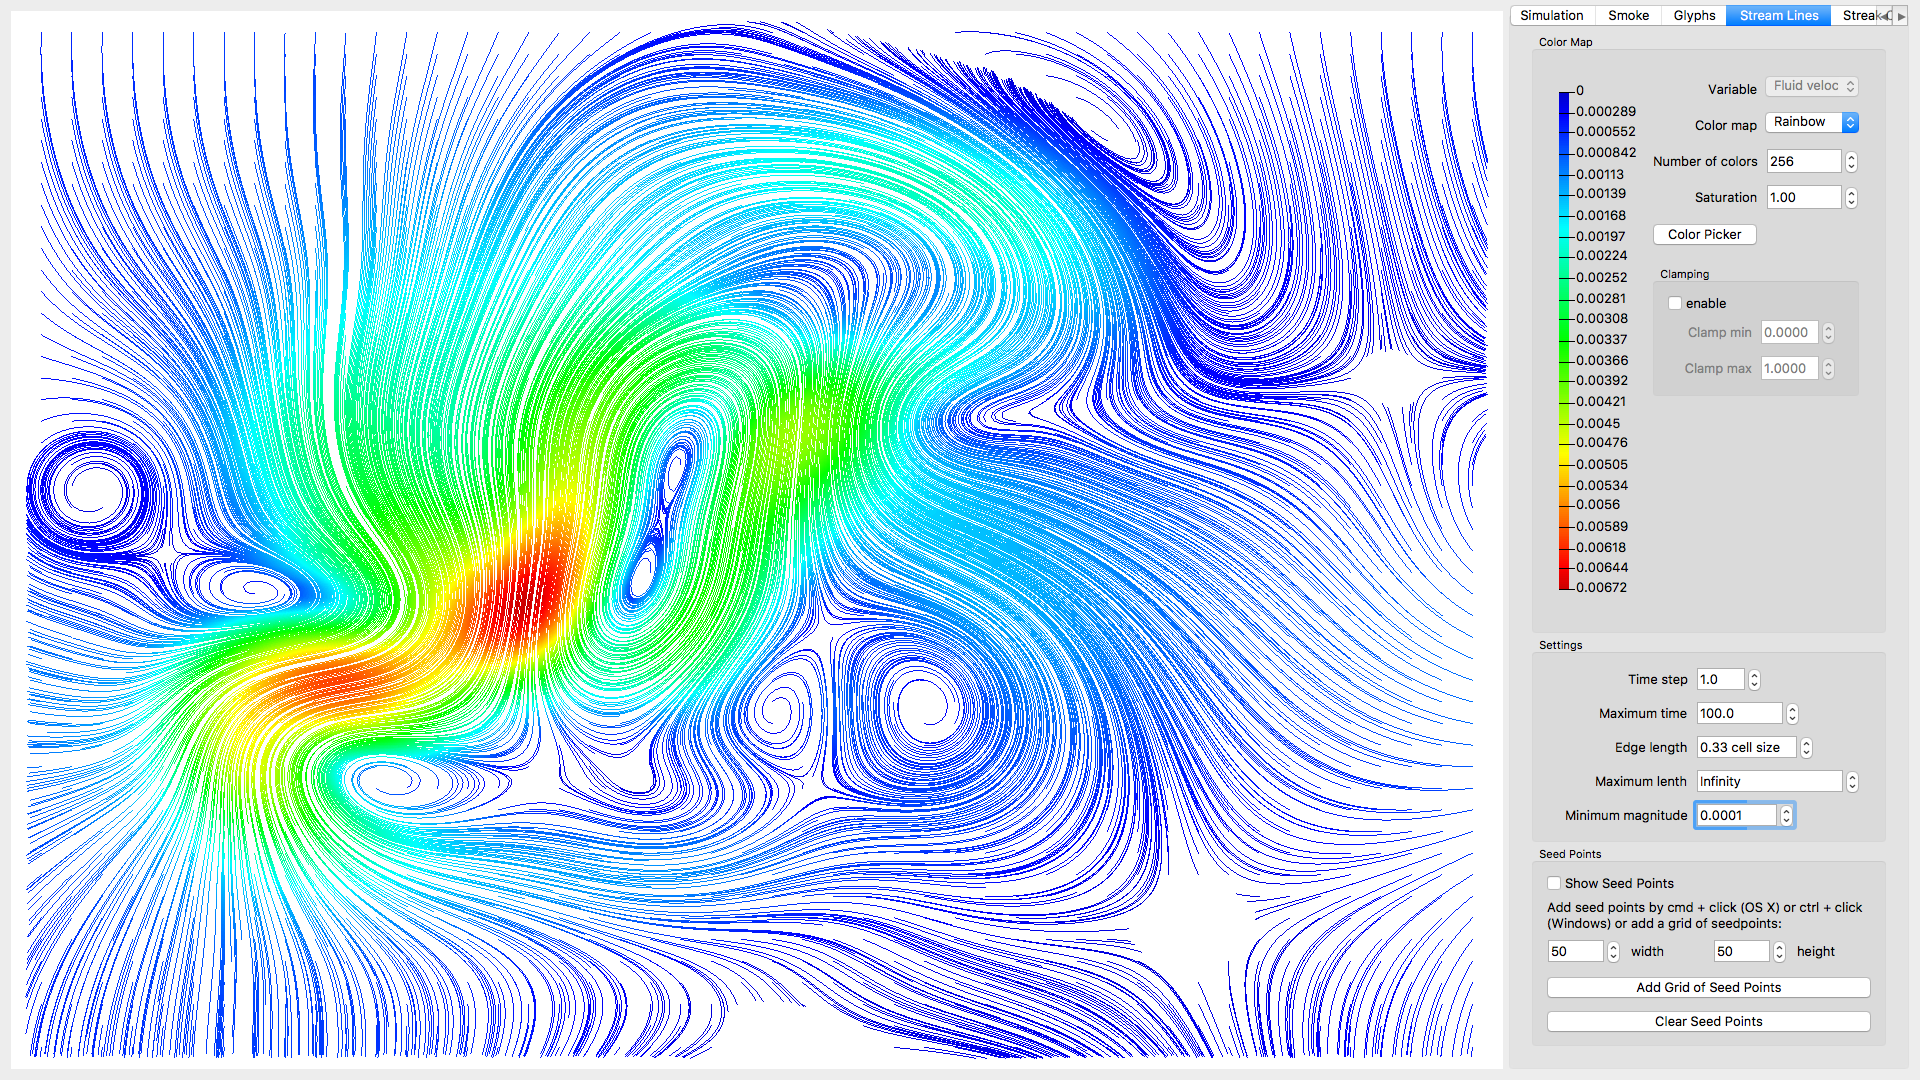
\includegraphics[width=0.42\textwidth, height=0.5\textheight, keepaspectratio=true]{img/titlepage/streamlines.png}

        \vspace{10px}
        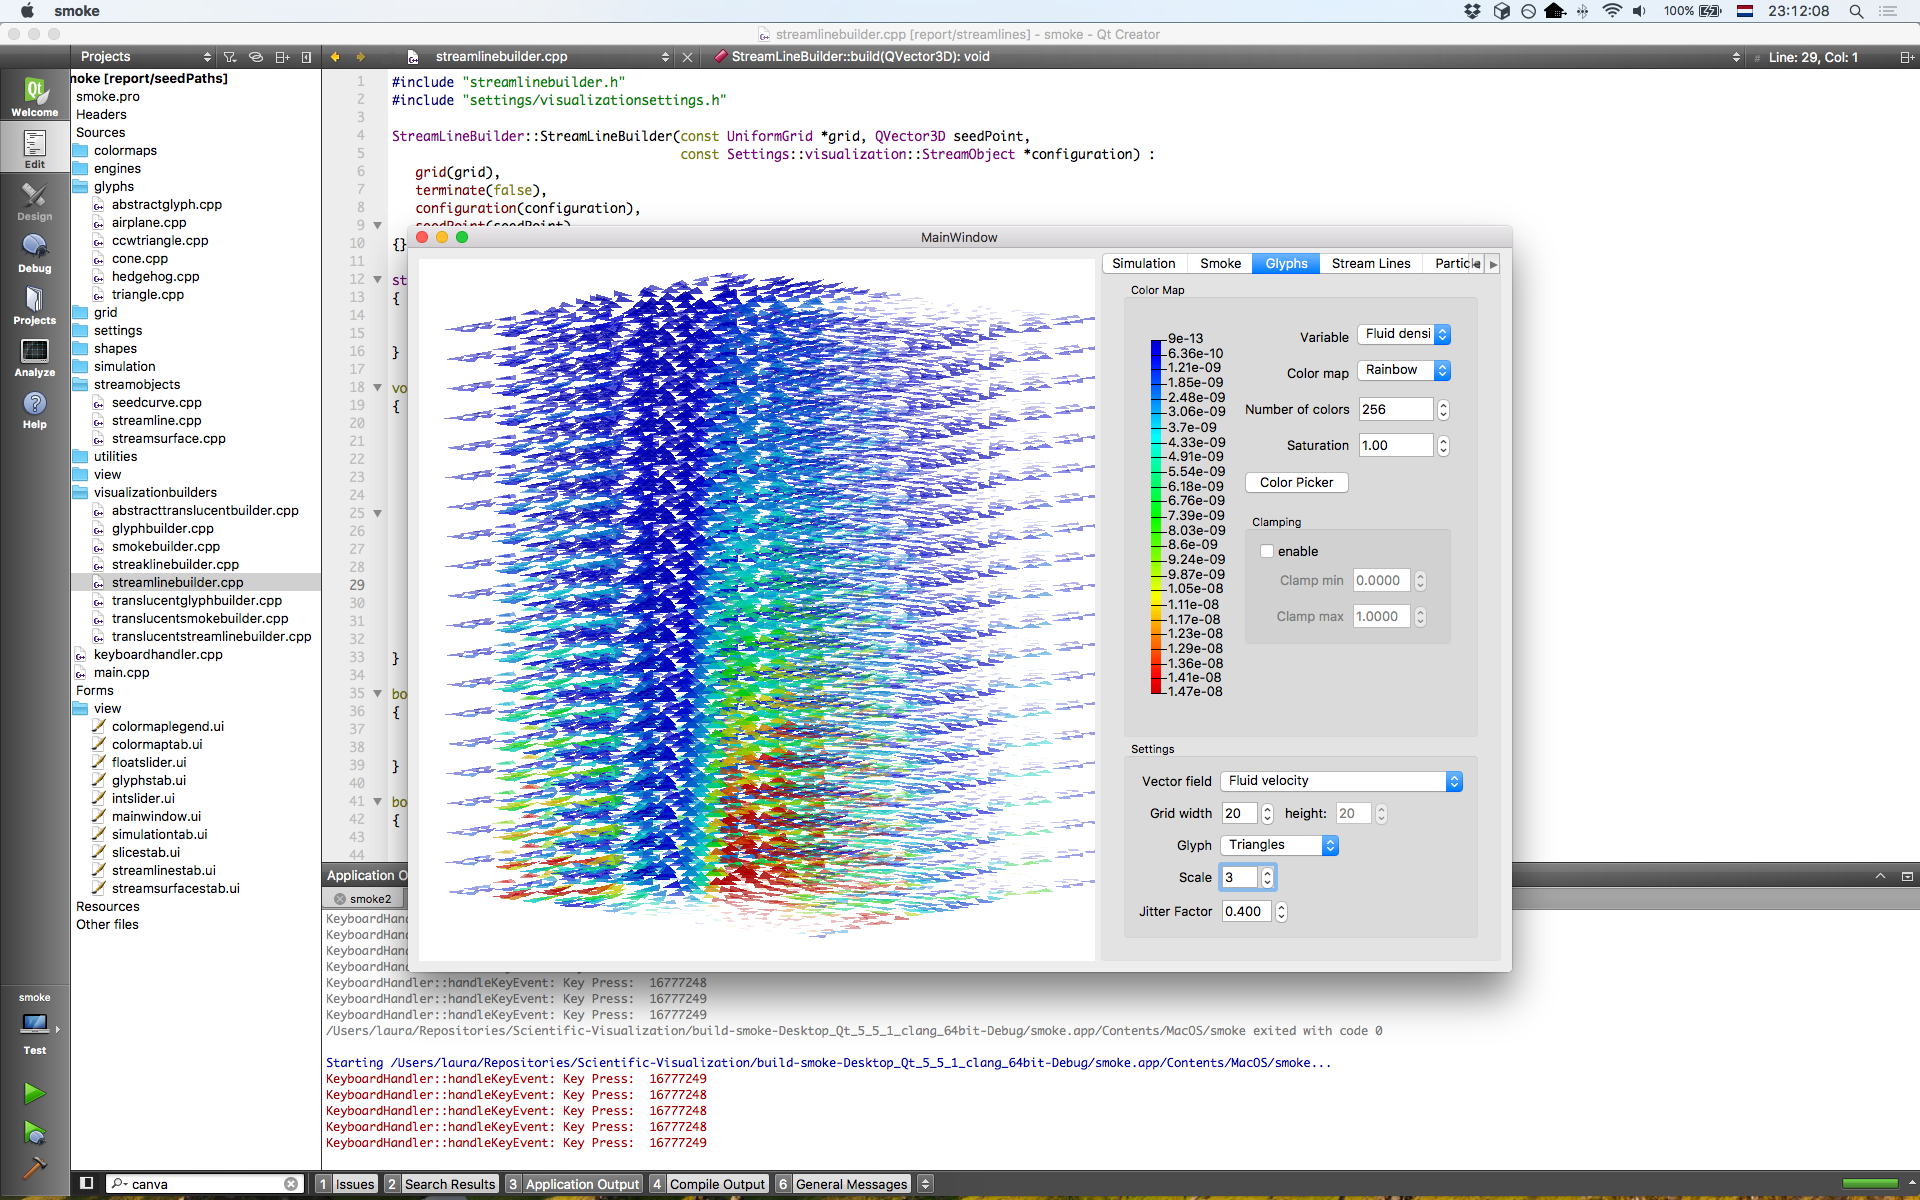
\includegraphics[width=0.42\textwidth, height=0.5\textheight, keepaspectratio=true]{img/titlepage/slices.png} \hspace{10px}
        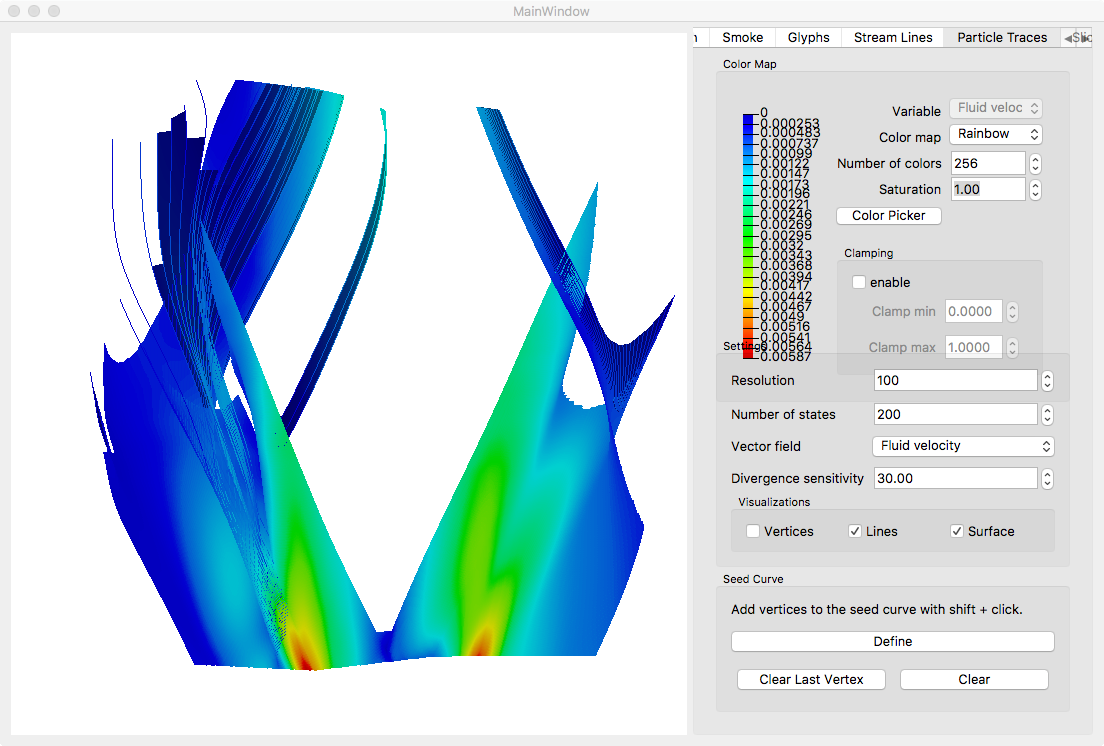
\includegraphics[width=0.42\textwidth, height=0.5\textheight, keepaspectratio=true]{img/titlepage/streamsurfaces.png}        
    \vspace{2cm}\par

    {\Large L.E.N. Baakman \textsc{s}1869140\par}
    {\Large S.J. van Loon \textsc{s}1795813\par}

    \vfill
% Bottom of the page
    {\large \today\par}
\end{titlepage}
\hypersetup{pageanchor=true}